\documentclass[11pt]{report}
\usepackage{amsmath}
\usepackage{amssymb}
\usepackage{amsfonts}
\usepackage{mathtools}
\usepackage{amsthm}
\usepackage{ragged2e}
\usepackage[hidelinks]{hyperref}
\usepackage{float}
\usepackage{pgf,tikz}
\usepackage[shortlabels]{enumitem}
\usepackage{color}
\usepackage{pgfplots}
\usepackage[margin = 1 in]{geometry}
\usepackage{mathrsfs}
\usetikzlibrary{arrows}
\usepackage{multicol}
\usepackage{fancyhdr}
\pagestyle{fancy}
\usepackage{multirow}
\usepackage{graphicx}
\usepackage{psfrag}
\usepackage{biblatex}
\addbibresource{hw5.bib}
\usepackage{listings}
\renewcommand{\footrulewidth}{0.4pt}

\newtheorem{theorem}{Theorem}[chapter]
\newtheorem{defn}{Definition}[chapter]
\newtheorem{lemma}{Lemma}[chapter]

\theoremstyle{definition}
\newtheorem{proposition}{Proposition}[chapter]
\newtheorem{remark}{Remark}[chapter]
\newtheorem{example}{Example}[chapter]

\DeclareMathOperator*{\argmin}{arg\,min}
\DeclareMathOperator*{\argmax}{arg\,max}

\newcommand{\user}{}
\newcommand{\xlr}[2]{#1 \left(#2\right)}
\newcommand{\clr}[2]{#1 \left\{ #2 \right\}}
\newcommand{\rank}{\mathrm{rank}}
\newcommand{\mat}[1]{\mathbf{#1}}
\lhead{ECE 530 - Fall 2023 at University of Illinois at Urbana-Champaign}
\rhead{HW5}
\lfoot{Author: \textcolor{red}{Eric Silk, esilk2}}
\rfoot{Due: Friday, Oct. 20th}
\begin{document}


\section*{The Burden of Stability}
\subsection*{Problem Statement}
Consider the scalar ordinary differential equation (ODE):
\begin{equation}
	\dot{x}(t) = f(t, x(t)) \coloneqq \lambda x(t)+(1-\lambda)\cos(t)-(1+\lambda)sin(t),\ x(0)=1
\end{equation}


The file run\_ODE.m provides a framework to run various different methods for
numerical integration of $(1)$ with step-size $h > 0$ over time $t\in[0,T=10]$.
Let $N=\lfloor Th\rfloor$, where the notation $\lfloor\cdot\rfloor$ stands for
the largest integer not exceeding z. Specifically, it computes a vector $(x_0 =
	x(0), x_1, \ldots, x_N )$, where $x_n$’s are the proxies for $x(t_n)$ computed
recursively via different methods with tn = nh. Define the average error of any
numerical integration method applied to this ODE as
\[ \mathcal{E}\coloneqq \frac{1}{N+1}\sum_{n=0}^{N}|x(t_n)-x_n| \]
Use code or other methods to generate the plots required below and answer the questions.
Please submit your code (at least for parts c and d).

\subsubsection*{a}
Show that the analytical solution of the DOE is given by $x(t)=\cos(t)+\sin(t)$.

\subsubsection*{b}
lot the result of numerical integration via forward Euler method with
$h=0.15,0.30,0.45$ over $[0,T]$ together with the analytical solution. Comment
how the average error for forward Euler $\mathcal{E}_{FE}$ varies with $h$.  Is
forward Euler method stable for all values of h you simulated?

\subsubsection*{c}
To implement backward Euler method for a given step-size h > 0, one needs to solve the nonlinear
equation
\[x_{n+1} \coloneqq x_n + hf(t_{n+1}, x_{n+1})\]
in each iteration $n\geq 0$. Implement Newton-Raphson to solve the equation $F(y)=0$ where
\[F(y)\coloneqq y-x_n-hf(t_{n+1},y)\]
starting from the forward Euler solution, given by $y^{(0)}\coloneqq x_n +
	hf(t_n,x_n)$.  Iterate until $|F(y)|<10^{-5}$.  For the same values of h used in
part (b), numerically integrate (1) using backward Euler method and plot the
results together with the analytical solution on the same graph. Comment how the
average error for backward Euler $\mathcal{E}_{BE}$ varies with $h$. Is backward
Euler method stable for all values of h you simulated?

\subsubsection*{d}
To implement the trapezoidal method with step-size $h>0$, one needs to solve the
nonlinear equation
\[x_{n+1}\coloneqq x_n + \frac{h}{2}[f(t_n,x_n)+f(t_{n+1},x_{n+1})]\]
in each iteration $n\geq 0$. Implement Newton-Raphson to solve the equation $F(y)=0$ with
\[ F(y)\coloneqq y-x_n-\frac{h}{2}[f(t_n,x_n)+f(t_{n+1},y)] \]
starting from the forward Euler solution given by $y^{(0)}\coloneqq x_n+hf(t_n,x_n)$.
Iterate until $|F(y)|<10^{-5}$. For the same values used in part (b), numerically
integrate (1) using the trapezoidal methond and plot the results together with the
analytical solution on the same graph. Comment how the average error for this method
varies with $h$. Is this method stable for the values of $h$ you've simulated?

\subsection*{Solution}
\subsubsection*{a}
\subsubsection*{b}
\begin{figure}[h]
	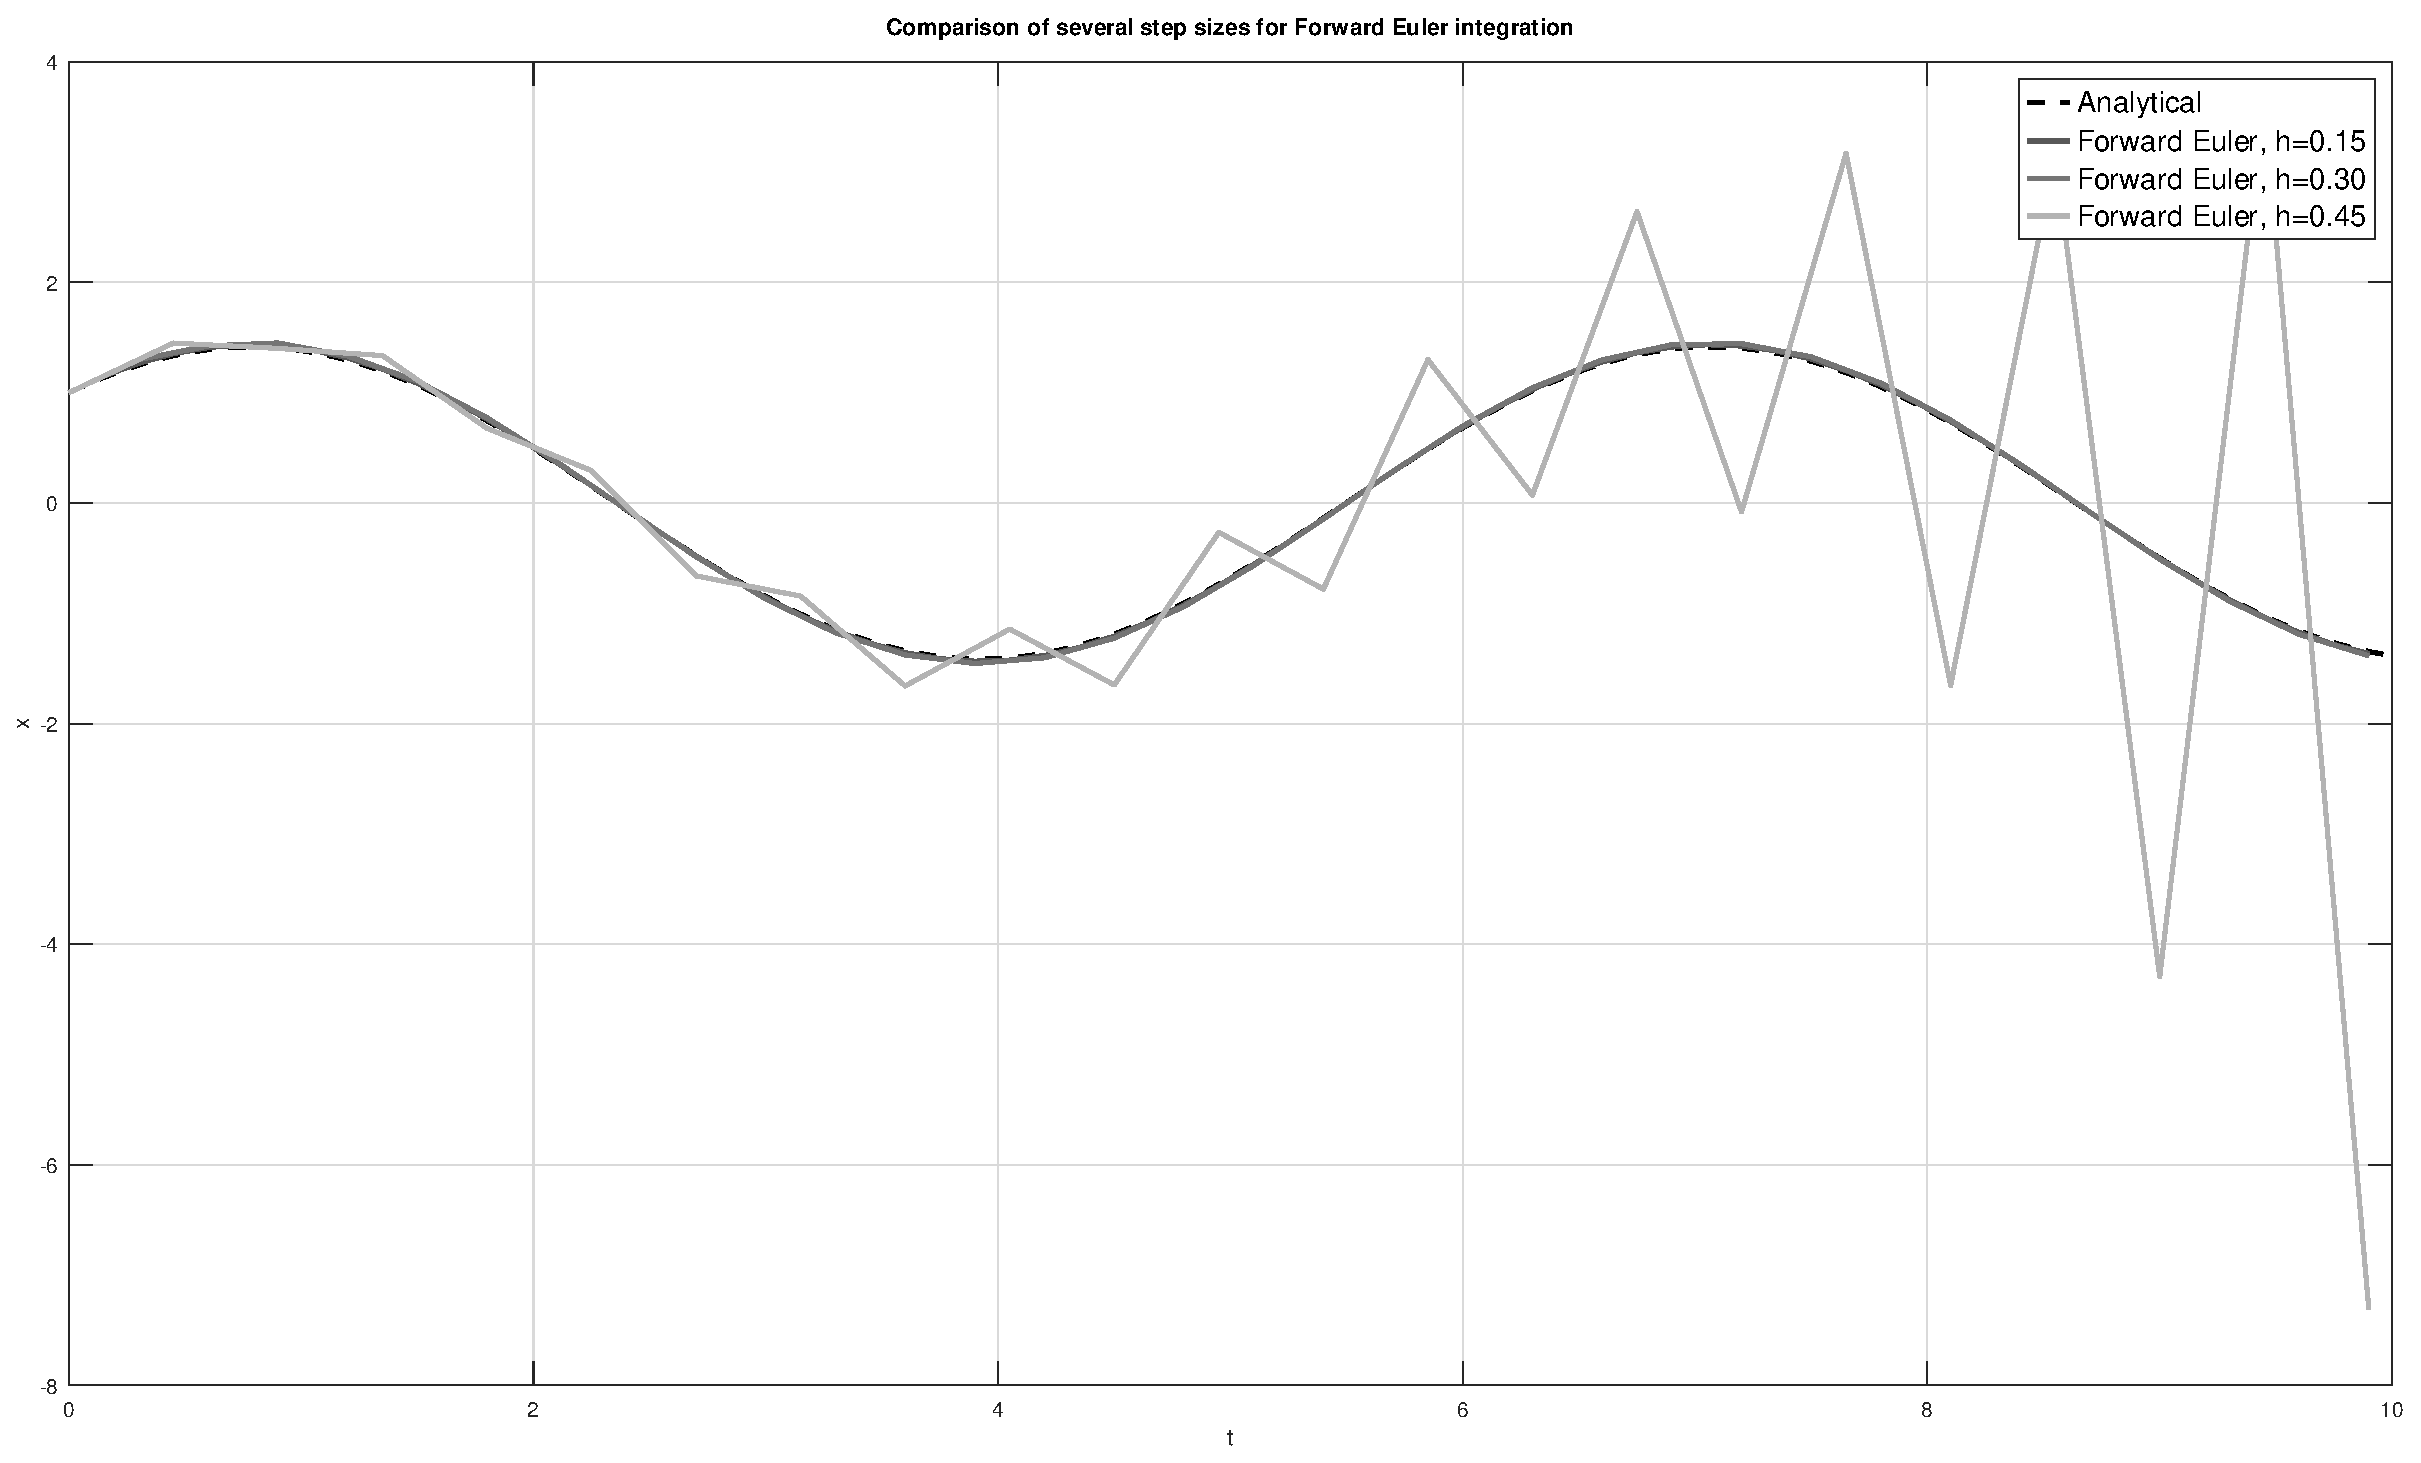
\includegraphics[width=\textwidth]{forward_euler}
\end{figure}
Mean error reported is 0.013344 for $h=0.15$, 0.027145 for $h=0.30$, and 1.2763
for $h=0.45$. Also, it is visually apparent that the solution for $h=0.45$
diverges, indicating numerical instability.
\subsubsection*{c, d}

\begin{lstlisting}[basicstyle=\small]
=======================================================================
h=0.1
Processing analytical solution.
Processing forward Euler method.
Mean error =0.0088783
Processing backward Euler method.
Mean error =0.086862
Processing trapezoidal method.
Mean error =0.085593
=======================================================================
h=0.15
Processing analytical solution.
Processing forward Euler method.
Mean error =0.013344
Processing backward Euler method.
Mean error =0.13035
Processing trapezoidal method.
Mean error =0.12856
=======================================================================
h=0.3
Processing analytical solution.
Processing forward Euler method.
Mean error =0.027145
Processing backward Euler method.
Mean error =0.25538
Processing trapezoidal method.
Mean error =0.25064
=======================================================================
h=0.45
Processing analytical solution.
Processing forward Euler method.
Mean error =1.2763
Processing backward Euler method.
Mean error =0.37076
Processing trapezoidal method.
Mean error =0.36708
\end{lstlisting}


\newpage
\section*{Problem 2: Conjugacy is Independence}
\subsection*{Problem Statement}
If $\{d^0,\ldots,d^{n-1}\}$ are pairwise $Q-$conjugate vectors in $\mathbb{R}^n\\\{0\}$
for $Q\succ0$ the prove they are linearly independent.

\subsection*{Solution}
Recall a sequence of vectors are linearly independent if:
\[\alpha_0d_0+\alpha_1d_0+\ldots+\alpha_kd_k=0\]
where not all scalars $\alpha_i=0$

If $\sum_{i=0}^{n-1}\alpha_i d_i$ then for $i_0\in{0,1,\ldots,n-1}$
\[ 0 = d^T_{i_0}Q\sum_{i=0}^{n-1}\alpha_i d_i = \alpha_{i_0}d_{i_0}^TQd_i \]
So $\alpha_i=0\forall i=0,\ldots,n-1$.
\qed

\noindent
Credit to Dr. Burke's website\cite{Burke_2007}.

\newpage
\section*{Problem 3: The Price of Laziness}
\subsection*{Problem Statement}
For the ODE given by $\dot{x}=f(x,t)$, investigate the absolute stability of the
following numerical integration schemes:
\begin{enumerate}
	\item Trapezoidal rule with one step fixed-point iteration from forward Euler, given by:
	      \[x_{n+1}=x_n+\frac{h}{2}[f(x_n,t_n)+f(x_n+hf(x_n,t_n), t_{n+1})]\]
	\item Backward Euler with one step fixed-point iteration from forward Euler, given by:
	      \[x_{n+1}=x_n+\frac{h}{2}f(x_n+hf(x_n,tn),t_{n+1})\]
\end{enumerate}

\subsection*{Solution}

\newpage
\section*{Code}
\definecolor{codegreen}{rgb}{0,0.6,0}
\definecolor{codegray}{rgb}{0.5,0.5,0.5}
\definecolor{codepurple}{rgb}{0.58,0,0.82}
\definecolor{backcolour}{rgb}{0.95,0.95,0.92}
\lstdefinestyle{mystyle}{
	backgroundcolor=\color{backcolour},
	commentstyle=\color{codegreen},
	keywordstyle=\color{magenta},
	numberstyle=\tiny\color{codegray},
	stringstyle=\color{codepurple},
	basicstyle=\ttfamily\footnotesize,
	breakatwhitespace=false,
	breaklines=true,
	captionpos=b,
	keepspaces=true,
	numbers=left,
	numbersep=5pt,
	showspaces=false,
	showstringspaces=false,
	showtabs=false,
	tabsize=2
}
\lstset{style=mystyle}
\lstinputlisting[
	language=MATLAB,
	basicstyle=\tiny
]{../../ece530/ece530/hw4/modifyHessian.m}
\lstinputlisting[
	language=MATLAB,
	basicstyle=\tiny
]{../../ece530/ece530/hw4/applyNewtonMethod.m}
%------------------------------------------------------------------------------------------------------------
\newpage
\printbibliography

%------------------------------------------------------------------------------------------------------------

\end{document}
